\documentclass[11pt]{article}

\usepackage[latin1]{inputenc}
\usepackage[a4paper,top=1in,left=1in,right=1in,bottom=1in]{geometry}
\usepackage[pdftex]{graphicx}
\usepackage{natbib}

\begin{document}

\pagestyle{empty}

\centerline{

\includegraphics[height=22mm]{Logos/logo_uga.png}
\hspace{5mm}

\includegraphics[height=22mm]{Logos/logo_cnrs.png}
\hfill

\includegraphics[height=22mm]{Logos/logo_ige.png}
}

\vspace{20mm}

\begin{center}

{\Huge\bf EnsScores}

\vspace{10mm}

{\Large\bf Ensemble Scores}

\vspace{10mm}

{\Large\bf User's guide}

\vspace{10mm}

{\large\bf Jean-Michel Brankart}

\vspace{5mm}
{\tt https://github.com/brankart/ensdam}

\vspace{5mm}
{\large Institut des G\'eosciences de l'Environnement}

\vspace{1mm}
{\large Universit\'e Grenoble Alpes, CNRS, France}

\end{center}

\vspace{20mm}
The purpose of EnsScores is to provide tools
to compute probabilistic scores for ensemble simulations.
The scores evaluate the reliability and/or the resolution of an ensemble simulation
by comparison to verification data.
For posterior ensembles (conditioned to observations),
there is also a score to evaluate the optimality of the result,
by testing its compatibility with observation uncertainty.

The tools are provided as a library of modules,
which can be easily plugged in an existing software.
This library includes:

\begin{itemize}
\item the computation of the Continuous Rank Probability Score (CRPS);
\item the computation of the Reduced Centered Random Variable (RCRV) score;
\item the computation of scores based on the relative entropy of user-defined events;
\item the computation of an optimality score for posterior ensembles.
\end{itemize}

\clearpage

\pagestyle{plain}

\section{Description of the methods}

The standard protocol to evaluate the performance of ensemble simulations
is to measure the {\em reliability} and the {\em resolution} of the ensemble
using {\em verification data} \citep{TOTH03,CAND05,CAND07}.
These scores can be used to compare ensemble forecasting systems,
ensemble analyses, or to evaluate the impact of observations in these systems
(using observation system simulation experiments).
In the case of a posterior ensemble (conditioned on observations),
it is also possible to check that the observations have been used optimally.
A necessary condition of {\em optimality} is indeed that the distance
between the observations and the ensemble members
is compatible with the probability distribution of observation errors.

\subsection{Reliability}

Reliability is a measure of the consistency between the ensemble and the verification data.
The idea is to check the hypothesis that the verification data
are drawn from the same probability distribution as the ensemble members.
For instance, a necessary condition of reliability is that
verification data have the same probability to fall in every interval
defined by the ensemble members.
This can be checked by drawing a {\em rank histogram} of the verification data \citep{ANDE96},
as used and described for instance in \citet{CAND15} or \citet{GARN16}, and
as can be computed by the {\tt\bf score\_ranks} module of this package.

To obtain a more compact score, we can center/reduce
the verification data with the ensemble mean and ensemble standard deviation.
A necessary condition of reliability (less stringent than the rank histogram) is then that
this Reduced Centered Random Variable (RCRV) has zero mean and unit standard deviation.
This is what is checked by the RCRV score \citep{CAND07},
as computed by the {\tt\bf score\_rcrv} module of this package.

The Continuous Rank Probability Score (CRPS),
as computed by the {\tt\bf score\_crps} module of this package,
also provides an evaluation of reliability
using the decomposition of the score into reliability and resolution,
as described in \citet{HERS00}: CRPS = Reli + Resol.
In this case, it is important to check that the reliability component
of the CRPS is much smaller than the resolution component.

Reliability is indeed the most important feature of an ensemble simulation.
There is no point having good resolution or optimality scores
if the ensemble is not reliable.

\subsection{Resolution}

Resolution is a measure of the accuracy of the ensemble,
or the amount of information that it provides about the system.
For instance, if the ensemble is perfectly reliable,
a small ensemble spread will provide a better resolution
than a large ensemble spread.

The Continuous Rank Probability Score (CRPS),
as computed by the {\tt\bf score\_crps} module of this package,
provides an evaluation of resolution that complements
the reliability component to explain the total CRPS score.
The total CRPS score is a measure of the misfit between the Cumulative Distribution Functions (cdf)
described by the ensemble (stepwise cdf) and the verification data (Heavside cdf).
The score is thus expressed in the unit of the input variable,
and the smaller the score, the better.
For a perfectly reliable ensemble (Reli=0), this misfit (i.e. the total CRPS score)
is only due to the ensemble spread.
For an ensemble without spread, this misfit is only due to a shift
between the zero-spread ensemble and the verification data
(a very bad reliability, unless this shift if zero).

Providing that reliability has been verified,
information theory can also provide means of evaluating
the resolution of an ensemble simulation
in terms of the amount of information that it provides about specific events \citep{ROUL02}.
From the probability distribution of an event described by the ensemble,
it is for instance possible to evaluate how much information
has been gained as compared to a climatological distribution
or as compared to a prior distribution.
This is the purpose of the  {\tt\bf score\_entropy} module of this package,
which implements the method described in \citet{GERM19}.
In this paper, the method was used in the context
of an Observation System Simulation Experiment,
to evaluate how much information was gained about specific events
for different quality of observation systems
(in terms of coverage and accuracy).

\subsection{Optimality}

When a prior ensemble is conditioned to observations
to produce a posterior ensemble,
what is expected from the observational update is
that the resolution can be improved (by the information brought
by the observations), without degrading reliability.
These scores tell us how much the updated ensemble has improved
as compared to the prior ensemble.
However, they do not tell us if we made the best possible use of the available observations.
Is the updated ensemble close enough to observations
to be consistent with the probability distribution of observation errors?

To evaluate this, we can use the optimality score proposed in \citet{BRAN19},
as implemented in the {\tt\bf score\_optimality} module of this package.
In short, this score is obtained by computing the rank~$r_{ij}^o$
of every observation~$y^o_j,\,j=1,\ldots,p$ in the probability
distribution for observation errors~$p(y^o_j|{\bf x}_i)$,
conditioned on every member~${\bf x}_i,\,i=1,\ldots,m$ of the ensemble.
If optimality is achieved, this rank is uniformly distributed between 0 and~1.
To obtain a single score, we transform this uniform number
into a ${\mathcal N}(0,1)$ number, and take the mean square.
This defines the optimality score, which is expected to be equal to~1
(for $p\rightarrow\infty$ and $m\rightarrow\infty$).

This score does not make any assumption on the probability distribution
described by the ensemble or on observation error probability distribution.
However, in the particular case of Gaussian distributions,
the score is equivalent to computing the mean square misfit between the observations
and all {\em individual ensemble members},
and check that the result is equal to the observation error variance.
In the Gaussian case, this mean square misfit can be decomposed as the sum
of the variance of the residual error (ensemble spread)
and the mean square observation misfit with the ensemble mean \citep{TALA99}.
The more observational information, the smaller the ensemble spread,
and the larger the observation misfit to the ensemble mean.
It is indeed the sum of these two components that must be equal to the observation error variance.
By looking at the misfit between observations and individual ensemble members (rather than the ensemble mean),
we can directly compare to the observation error distribution
and generalize the optimality check to non-Gaussian distributions.

\subsection{About verification data}

In the above discussion about reliability and resolution,
it was assumed that the verification data are error free,
as can be the case in twin assimilation experiments or
in observation system simulation experiments.
In this case, the reliability of the ensemble
can be evaluated directly using the modules provided in this package.

However, if the verification data are observations,
the observation equivalent of the ensemble members
must be perturbed with a random observation error
before checking reliability (with a rank histogram or the RCRV score).
This can be very important if observation errors are not negligible
as compared to the spread of the ensemble.

\clearpage

\section{Description of the modules}

In this section,
the modules are described one by one,
giving for each of them:
the method that has been implemented,
the list of public variables and public routines
(with a description of input and output data),
the MPI parallelization, and
an estimation of the computational cost
as a function of the size of the problem.

\subsection{Module: {\tt\bf score\_ranks}}

The purpose of this module is to compute the rank
of the verification data in the ensemble simulation
and to produce a rank histogram.

\subsubsection*{Method}

The algorithm loops on the verification data,
sort the ensemble members for each of them,
and compute the rank of each element of the verification data
within the sorted ensemble values.
From the vector of ranks, a rank histogram is produced.

\subsubsection*{Public variables}

\begin{description}
\item[mpi\_comm\_score\_ranks:] MPI communicator to use (default=mpi\_comm\_world).
\end{description}

\subsubsection*{Public routines}

\begin{description}
\item[compute\_ranks:] compute CRPS score (with an option to partition the data
                    and compute the score for each subset of data):
  \begin{description}
  \item[{\tt ens} (input)]: ensemble to evaluate (model equivalent to verification data);
  \item[{\tt verif} (input)]: verification data;
  \item[{\tt ranks} (output)]: ranks of the verification data within the ensemble;
  \item[{\tt rank\_histogram} (output, optional)]: rank histogram.
  \end{description}
\end{description}

\subsubsection*{MPI parallelization}

Parallelization is obtained by making each processor call the routine
for a different chunk of the verification data.
The routine combines the contributions from all processors
to compute a global rank histogram.

\subsubsection*{Computational cost}

The cost mainly results from the sorting of the ensemble members
for each variable in the verification data.
It is thus proportional to $n m \log_2 m$,
if $m$ is the size of the ensemble and $n$, the size of the verification dataset.

\subsection{Module: {\tt\bf score\_crps}}

The purpose of this module is to compute the CRPS
of an ensemble simulation by comparison to verification data.

\subsubsection*{Method}

The total CRPS score corresponds to the misfit between two probability distributions
of a one-dimensional random variable~$x$ is the area
between their respective cumulative distribution functions (cdf)
$F(x)$ and~$F_{\mbox{ref}}(x)$:

\begin{equation}
\label{eq:crps}
\Delta = \int_{-\infty}^{\infty}
\left| F(x) - F_{\mbox{ref}}(x) \right| \; dx
\end{equation}

\noindent
In our case, the reference cdf~$F_{\mbox{ref}}(x)$
is a Heaviside function increasing by~1
at the true value of the variable,
and the ensemble cdf~$F(x)$ is a stepwise function
increasing by~$1/m$ at each of the ensemble values
(where $m$ is the size of the ensemble).
This is illustrated in Fig.~\ref{fig:crps},
where $\Delta$ is the blue area between the two cdfs.
The further the ensemble values from the reference,
the larger~$\Delta$, and the unit of~$\Delta$
is the same as the unit of~$x$.

\begin{figure}[htbp]
\centerline{
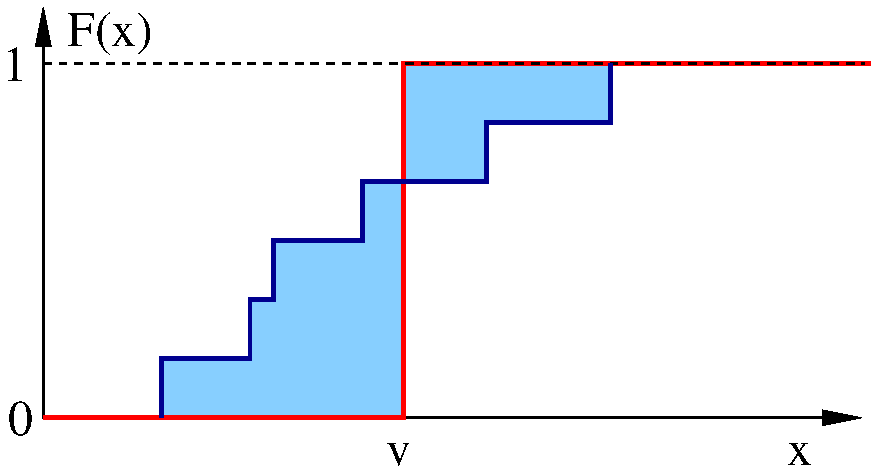
\includegraphics[width=0.7\textwidth]{Figures/ensscores_crps.pdf}
}
\caption{Illustration of the CRPS score.
The reference cdf is in red;
The ensemble cdf (6~members) is in dark blue;
and the CRPS score is the blue area between the two cdfs.
\label{fig:crps}}
\end{figure}

The algorithm in the routines loops on the verification data,
to accumulate the contribution of each of them
(in the intermediate arrays {\tt aa} and {\tt bb}),
and then compute the overal CRPS score,
together with the reliability and resolution components.

\subsubsection*{Public variables}

\begin{description}
\item[mpi\_comm\_score\_crps:] MPI communicator to use (default=mpi\_comm\_world).
\item[crps\_missing\_value:] missing value to use where no data is available (default=-9999.).
\end{description}

\subsubsection*{Public routines}

\begin{description}
\item[crps\_score:] compute CRPS score (with an option to partition the data
                    and compute the score for each subset of data):
  \begin{description}
  \item[{\tt crps} (output)]: CRPS score for each subset of data;
  \item[{\tt reliability} (output)]: reliability part of CRPS;
  \item[{\tt resolution} (output)]: resolution part of CRPS;
  \item[{\tt ens} (input)]: ensemble to evaluate (model equivalent to verification data);
  \item[{\tt verif} (input)]: verification data;
  \item[{\tt partition} (input, optional)]: partition of verification data
                                  (giving the index of the subset for each element of the data).
  \end{description}
\item[crps\_cumul:] accumulate data to prepare the final computation of the score
                    (for advanced use, if the full ensemble is only made progressively available).
\item[crps\_final:] compute final score from accumulated data
                    (for advanced use, if the full ensemble is only made progressively available).
\end{description}

\subsubsection*{MPI parallelization}

Parallelization is obtained by making each processor call the routine
for a different chunk of the verification data.
The routine combines the contributions from all processors
to compute a global score.

\subsubsection*{Computational cost}

The cost mainly results from the sorting of the ensemble members
for each variable in the verification data.
It is thus proportional to $n m \log_2 m$,
if $m$ is the size of the ensemble and $n$, the size of the verification dataset.

\subsection{Module: {\tt\bf score\_rcrv}}

The purpose of this module is to compute the RCRV
of an ensemble simulation by comparison to verification data.

\subsubsection*{Method}

The Reduced Centered Random Variable (RCRV) is defined from

\begin{equation}
 \label{eq:rcrv}
  y = \frac{v-m}{\sigma}
\end{equation}

\noindent
where $v$  is one of the verification data and
$m$ and $\sigma$ are the corresponding mean and the standard deviation of the ensemble.
The system is reliable, if the mean of $y$ over all realisations
is equal to zero and its standard deviation is equal to 1.
Thus, the reliability is decomposed into (normalized) bias $b=E[y]$
and dispersion $d^2=E[y^2]-b^2$, which are the two quantities
provided by this module.

To compute the score, the algorithm in the routine loops on the verification data,
to accumulate the contribution of each of them
(to the reduced bias and reduce spread),
and then compute the overal RCRV score
(bias component and spread component).
If the anamorphosis option is activated (see below),
the reduced variable (zero mean, unit standard deviation, Gaussian distribution)
is obtained by anamorphosis (using quantiles of the input ensemble)
rather than center/reduction (using the ensemble mean and standard deviation).

\subsubsection*{Public variables}

\begin{description}
\item[mpi\_comm\_score\_rcrv:] MPI communicator to use (default=mpi\_comm\_world).
\item[rcrv\_missing\_value:] missing value to use where no data is available (default=-9999.).
\item[rcrv\_with\_anamorphosis:] use anamorphosis to compute reduced variable (default=.FALSE.).
\item[rcrv\_number\_of\_quantiles:] number of quantiles to perform anamorphosis (default=11).
\end{description}

\subsubsection*{Public routines}

\begin{description}
\item[rcrv\_score:] compute RCRV score (with an option to partition the data
                    and compute the score for each subset of data):
  \begin{description}
  \item[{\tt ens\_bias} (output)]: bias component of RCRV (should be 0);
  \item[{\tt ens\_spread} (output)]: spread component of RCRV (should be 1);
  \item[{\tt ens} (input)]: ensemble to evaluate (model equivalent to verification data);
  \item[{\tt verif} (input)]: verification data.
  \item[{\tt partition} (input, optional)]: partition of verification data
                                  (giving the index of the subset for each element of the data).
  \end{description}
\item[rcrv\_cumul:] accumulate data to prepare the final computation of the score
                    (for advanced use, if the full ensemble is only made progressively available).
\end{description}

\subsubsection*{MPI parallelization}

Parallelization is obtained by making each processor call the routine
for a different chunk of the verification data.
The routine combines the contributions from all processors
to compute a global score.

\subsubsection*{Computational cost}

Without anamorphosis, the cost grows linearly with the ensemble size ($m$)
and the size of the verification dataset ($n$).
It is thus proportional to $n m$.

\noindent
With anamorphosis, the cost mainly results from the sorting of the ensemble members
for each variable in the verification data (to compute the quantiles).
It is thus proportional to $n m \log_2 m$.

\subsection{Module: {\tt\bf score\_entropy}}

The purpose of this module is to compute
scores based on the relative entropy of user-defined events.

\subsubsection*{Method}

To use this module, the user must provide a routine
computing the outcome of one or several events from a given ensemble member.
It is provided as the callback routine {\tt events\_outcome} (see below).
The events must be discrete, with a finite number of possible outcomes
({\tt jpo}, which should be much smaller than the ensemble size).
The callback routine must provide the index of the outcome (between 1 and {\tt jpo}) for each event.
From this routine, the module can then compute:

\begin{itemize}
\item the probability distribution of the events in a given ensemble (routine {\tt events\_probability}):
this is just computed as the number of members with a given outcome, divided by the size of the ensemble;
\item the entropy associated to each event in a given ensemble (routine {\tt events\_entropy}),
which can be directly computed from the probability distribution;
\item the cross entropy between the ensemble distribution and a reference distribution
provided by the user (routine {\tt events\_cross\_entropy});
\item the relative entropy between the ensemble distribution and a reference distribution
provided by the user (routine {\tt events\_relative\_entropy});
\item a score (between 0 and 1) describing the gain obtained for each event,
as compared to the reference distribution (routine {\tt events\_scores}),
which is computed as the ratio between entropy and cross entropy.
\end{itemize}

\noindent
For example, the reference distribution can be a climatological distribution or a prior distribution.
The score describes the gain in resolution provided by the ensemble as compared to this distribution.

\subsubsection*{Public variables}

\begin{description}
\item[score\_entropy\_base:] base to use in the computation of logarithms (default=2.).
\end{description}

\subsubsection*{Public routines}

\begin{description}
\item[events\_score:] compute entropy based score:
  \begin{description}
  \item[{\tt score} (output)]: ensemble score for each event;
  \item[{\tt ens} (input)]: ensemble to evaluate;
  \item[{\tt pref} (input)]: reference probability distribution for each event;
  \item[{\tt events\_outcome} (input)]: callback routine providing the outcome
                                        of the events for a given member.
  \end{description}
\item[events\_relative\_entropy:] compute relative entropy:
  \begin{description}
  \item[{\tt relative\_entropy} (output)]: relative entropy (with respect to reference distribution);
  \item[{\tt ens} (input)]: ensemble to evaluate;
  \item[{\tt pref} (input)]: reference probability distribution for each event;
  \item[{\tt events\_outcome} (input)]: callback routine providing the outcome
                                        of the events for a given member.
  \end{description}
\item[events\_cross\_entropy:] compute cross entropy:
  \begin{description}
  \item[{\tt cross\_entropy} (output)]: cross entropy (with reference distribution);
  \item[{\tt ens} (input)]: ensemble to evaluate;
  \item[{\tt pref} (input)]: reference probability distribution for each event;
  \item[{\tt events\_outcome} (input)]: callback routine providing the outcome
                                        of the events for a given member.
  \end{description}
\item[events\_entropy:] compute ensemble entropy:
  \begin{description}
  \item[{\tt entropy} (output)]: ensemble entropy;
  \item[{\tt number\_outcome} (input)]: number of possible outcomes for the events;
  \item[{\tt ens} (input)]: ensemble to evaluate;
  \item[{\tt events\_outcome} (input)]: callback routine providing the outcome
                                        of the events for a given member.
  \end{description}
\item[events\_probability:] compute events marginal probability distributions from the ensemble:
  \begin{description}
  \item[{\tt pens} (output)]: ensemble probability distribution for each event;
  \item[{\tt ens} (input)]: ensemble to evaluate;
  \item[{\tt events\_outcome} (input)]: callback routine providing the outcome
                                        of the events for a given member.
  \end{description}
\end{description}

\subsubsection*{MPI parallelization}

No parallelization is implemented.

\subsubsection*{Computational cost}

The cost mainly depends on the evaluation of the outcome of an event
in the callback routine provided by the user.
This routine is called for each ensemble member.

\subsection{Module: {\tt\bf score\_optimality}}

The purpose of this module is to compute a score
evaluating the optimality of a posterior ensemble
by comparison to observations.

\subsubsection*{Method}

The algorithm loops on the observation data
to accumulate the contribution of each of them
(a `normalized distance' between each observation and each ensemble member)
and then compute the overal optimality score,
whose expected value must be equal to~1 for an optimal system.

The computation of this `normalized distance' requires an evaluation
of the observation error cdf (to compute the rank of the observation)
and the inverse Gaussian cdf (to tranform this rank into a Gaussian number).
In the case of Gaussian observation errors, this computation is simplified
by computing the difference between each observation and each ensemble member,
divided by the observation error standard deviation.

It must be noted that this score is only a necessary condition of optimality,
focusing on the testing of the marginal probability distributions.
It can thus be computed whether observation errors are correlated or not.
However, the convergence to the expected value of the score
will depend on the number of degrees of freedom in the observations.

\subsubsection*{Public variables}

\begin{description}
\item[mpi\_comm\_score\_optimality:] MPI communicator to use (default=mpi\_comm\_world).
\item[optimality\_missing\_value:] missing value to use where no data is available (default=-9999.).
\end{description}

\subsubsection*{Public routines}

\begin{description}
\item[optimality\_score:] compute optimality score (with an option to partition the data
                    and compute the score for each subset of data):
  \begin{description}
  \item[{\tt ens\_optimality} (output)]: optimality score (should be 1);
  \item[{\tt ens} (input)]: ensemble to evaluate (model equivalent to observations);
  \item[{\tt obs} (input)]: observation data;
  \item[{\tt partition} (input, optional)]: partition of observation data
                                  (giving the index of the subset for each element of the data);
  \item[{\tt std\_obs} or {\tt obs\_cdf} (input)]: standard deviation of observation errors
                            (in the case of Gaussian observation errors) or
                            callback routine providing the cdf of observation errors
                            (in the case of non-Gaussian observation errors).
  \end{description}
\item[optimality\_cumul:] accumulate data to prepare the final computation of the score
                    (for advanced use, if the full ensemble is only made progressively available).
\end{description}

\subsubsection*{MPI parallelization}

Parallelization is obtained by making each processor call the routine
for a different chunk of the verification data.
The routine combines the contributions from all processors
to compute a global score.

\subsubsection*{Computational cost}

The cost mainly depends on the evaluation of the observation error cdf
(callback routine provided by the user) and the inverse Gaussian cdf.
The number of calls of these two routines is $n m$,
where $n$ is the number of observations and $m$, the ensemble size.

\clearpage

\section{Examples}

Two examples are provided to illustrate these modules:
(i)~a very simple idealized example illustrating how to call the routines,
and how the results can depend on the number of verification data or the size of the ensemble, and
(ii)~a more sophisticated example, which corresponds to the use of these modules
to evaluate the MCMC sampler in \citet{BRAN19}.

\subsection{A simple idealized test case}

The code for this example is {\tt\bf score\_idealized\_example}.
It illustrates all score modules: {\tt\bf scor\_crps}, {\tt\bf scor\_rcrv},
{\tt\bf scor\_entropy} and {\tt\bf scor\_optimality}.

In this example, a synthetic ensemble is generated
by sampling independent Gaussian random numbers
with zero mean and unit standard deviation.
The size of the state vector is~$n=1000$ and the ensemble size is~$m=100$.
The use of independent variables is overly simplistic,
but it is sufficient to illustrate the computation of the scores,
since all methods proceed in the same way
whether the variables are independent or not.

One additional ensemble member is drawn from the same distribution
to be used as the reference truth.
This reference truth is used to generate one pseudo-observation
for each of the variables, with an error standard deviation equal to~$\sigma=0.3$.
A posterior ensemble is then computed by conditioning the prior ensemble
to these pseudo-observations.

All modules are then used to evaluate the reliability, resolution
and optimality of the prior and posterior ensemble,
using the reference truth as verification data for reliability and resolution.
It is then easy to see how the statistics of the scores
can change with $n$, $m$ and~$\sigma$ in the case of independent variables.
One can also check how the score deteriorates
when the reference truth is sampled from a distribution
that is different from the prior ensemble, or
when the observational update is made non-optimal
(for instance using a wrong parameterization of observation errors).

Two events that can occur in the ensemble members
will be used to illustrate the behaviour of the entropy score:

\begin{enumerate}
\item The first event is defined from the mean square of the ensemble member: above or below~1.
In a real system, this could be the energy in the system above or below a user-requested level.
\item The second event is defined from the maximum absolute value of the ensemble member: above or below~3.3.
In a real system, this could be the occurence of an extreme event above or below a user-requested level.
\end{enumerate}

\noindent
These are two binary events which have two outcomes
with a similar probability (close to 0.5) in the prior ensemble.
There is thus no much prior information about them,
and we can check how much information
can be gained by the observations.

\begin{itemize}
\item
With the default setting of the example code
($m=100$, $n=1000$ and $\sigma=0.3$)
and with an optimal observational update,
the output of the example is the following:

\begin{verbatim}
Prior CRPS reliability and resolution:     0.00104 0.56067
Posterior CRPS reliability and resolution: 0.00030 0.16223
Prior RCRV bias and spread:      0.02900  0.99723
Posterior RCRV bias and spread: -0.03375  1.00673
Prior probability distribution (event 1):     0.480 0.520
Prior probability distribution (event 2):     0.450 0.550
Posterior probability distribution (event 1): 0.810 0.190
Posterior probability distribution (event 2): 0.900 0.100
Entropy score (posterior vs prior, event 1): 0.676
Entropy score (posterior vs prior, event 2): 0.418
Prior optimality score:     4.81227
Posterior optimality score: 1.00351
\end{verbatim}

We see that the reliability score is good in the prior ensemble (by construction),
and that it does not get worse after the observational update (posterior ensemble).
The resolution of the ensemble has been improved by the observations:
the CRPS resolution is smaller in the posterior ensemble,
and the entropy score also shows an improvement (score well below 1).
The probability concentrates on the first outcome of the two events.
The optimality score decreases to~1, which means that the ensemble members
are moved to the right typical 'distance' from the observations.

\item
If we decrease the observation error standard deviation
with respect to the default setting to $\sigma=0.05$,
the output of the example is the following:

\begin{verbatim}
Prior CRPS reliability and resolution:     0.00104 0.56067
Posterior CRPS reliability and resolution: 0.00006 0.02847
Prior RCRV bias and spread:      0.02900  0.99723
Posterior RCRV bias and spread: -0.04206  1.01476
Prior probability distribution (event 1):     0.480 0.520
Prior probability distribution (event 2):     0.450 0.550
Posterior probability distribution (event 1): 1.000 0.000
Posterior probability distribution (event 2): 1.000 0.000
Entropy score (posterior vs prior, event 1): 0.000
Entropy score (posterior vs prior, event 2): 0.000
Prior optimality score:    28.12474
Posterior optimality score: 1.00250
\end{verbatim}

Reliability and optimality are still good.
Resolution has strongly improved
by the much better information provided by the observations.
Entropy has decreased to zero for the two events:
all posterior members have the same outcome for each of them.
Uncertainty about them has been removed by the observations
(or, more precisely, the remaining uncertainty is too small
to be resolved by a 100-member ensemble).

\item
Starting again from the default setting,
we now modify the ensemble observational update algorithm
by omitting the perturbations applied to the observations
to perform the update of each ensemble member.

\begin{verbatim}
Prior CRPS reliability and resolution:     0.00104 0.56067
Posterior CRPS reliability and resolution: 0.03838 0.15373
Prior RCRV bias and spread:      0.02900  0.99723
Posterior RCRV bias and spread: -0.12757  3.46117
Prior probability distribution (event 1):     0.480 0.520
Prior probability distribution (event 2):     0.450 0.550
Posterior probability distribution (event 1): 1.000 0.000
Posterior probability distribution (event 2): 1.000 0.000
Entropy score (posterior vs prior, event 1): 0.000
Entropy score (posterior vs prior, event 2): 0.000
Prior optimality score:     4.81227
Posterior optimality score: 0.40346
\end{verbatim}

In this case, the scheme is wrong, and we can see this in the scores.
Reliability and optimality of the posterior ensemble have been lost.
The posterior ensemble is no more compatible with the reference truth
(e.g.~RCRV spread = $3.46 \gg 1$), and it is too close
to the observations (optimality score = $0.4 \ll 1$).
Resolution is apparently improved (in the CRPS and entropy scores),
but it does not serve any purpose since reliability is lost.

\end{itemize}

\subsection{Evaluation of the MCMC sampler}

The code for this example is {\tt\bf mcmc\_ensemble\_update}.
It uses the score modules: {\tt\bf scor\_crps} and {\tt\bf scor\_optimality}.

This code is an implementation of the work done in \citet{BRAN19}.
Refer to this paper to understand what is done in the code.

The score modules are used to evaluate the ensemble
that results from the application of the MCMC sampler.
Calls to the routines to evaluate reliability, resolution and optimality
of the ensemble can be found in the code and the results
are displayed in the figures of the paper.

\clearpage

\begin{thebibliography}{}

\bibitem[{Anderson(1996)}]{ANDE96}
Anderson J. 1996. A method for producing and evaluating probabilistic forecasts from ensemble model integrations. {\it J. Climate}, {\bf 9}, 1518--1530.

\bibitem[Brankart(2019)]{BRAN19}
Brankart J.-M., 2019:
Implicitly Localized MCMC Sampler to Cope
With Non-local/Non-linear Data Constraints in Large-Size Inverse Problems.
\textit{Front. Appl. Math. Stat.}, 5:58.

\bibitem[{Candille and Talagrand(2005)}]{CAND05}
Candille G., and O. Talagrand, 2005:
Evaluation of probabilistic prediction systems for a scalar variable.
{\it Quart. J. Roy. Meteor. Soc.}, {\bf 131}, 2131--2150.

\bibitem[Candille et al.(2007)]{CAND07}
Candille G., C. C\^ot\'e, P. L. Houtekamer, and G. Pellerin, 2007:
Verification of an ensemble prediction system against observations.
{\it Mon. Wea. Rev.}, {\bf 135}, 2688--2699.

\bibitem[Candille et al.(2015)]{CAND15}
Candille G., J.-M. Brankart, and P. Brasseur, 2015:
Assessment of an ensemble system that assimilates Jason-1/Envisat altimeter data
in a probabilistic model of the North Atlantic ocean circulation.
\textit{Ocean Science}, \textbf{11}, 425--438.

\bibitem[Garnier et al.(2016)]{GARN16}
Garnier F., J.-M. Brankart, P. Brasseur and E. Cosme, 2016:
Stochastic parameterizations of biogeochemical uncertainties
in a 1/4$^\circ$ NEMO/PISCES model for probabilistic comparisons
with ocean color data.
\textit{Journal of Marine Systems}, \textbf{155}, 59--72.

\bibitem[Germineaud et al.(2019)]{GERM19}
Germineaud, C., J.-M. Brankart, and P. Brasseur, 2019: An Ensemble-Based Probabilistic Score Approach to Compare Observation Scenarios: An Application to Biogeochemical-Argo Deployments. J. Atmos. Oceanic Technol., 36, 2307-2326.

\bibitem[{Hersbach(2000)}]{HERS00}
Hersbach H., 2000:
Decomposition of the continuous ranked probability score for ensemble prediction systems.
\textit{Wea. Forecasting}, \textbf{15}, 559--570.

\bibitem[{Roulston and Smith(2002)}]{ROUL02}
Roulston M. S. and L. Smith, 2002. Evaluating probabilistic forecast using information theory. {\it Mon. Wea. Review}, {\bf 130}, 1653--1660.

\bibitem[Talagrand(1999)]{TALA99}
Talagrand, O., 1999:
A posteriori verification of analysis and assimilation algorithms,
in: Workshop on diagnosis of data assimilation systems,
2--4 November 1998, ECMWF, Reading, UK, 1999.

\bibitem[Toth et al.(2003)]{TOTH03}
Toth Z., O. Talagrand, G. Candille, and Y. Zhu. 2003. Probability and ensemble forecasts,  in Forecast Verification: A Practitioner's Guide in Atmospheric Science, Jolliffe I. and D. B. Stephenson (eds), Wiley: UK. ISBN: 0-471-49 759-2, 137--163.

\end{thebibliography}

\end{document}

